\clearpage
\makeatletter
\efloat@restorefloats
\makeatother


\begin{appendix}
\renewcommand{\appendixname}{Supplementary Materials}
\renewcommand{\thefigure}{S\arabic{figure}} \setcounter{figure}{0}
\renewcommand{\thetable}{S\arabic{table}} \setcounter{table}{0}
\renewcommand{\theequation}{S\arabic{table}} \setcounter{equation}{0}

\hypertarget{section}{%
\section{}\label{section}}

\hypertarget{supplementary-methods}{%
\subsection{Supplementary Methods}\label{supplementary-methods}}

\hypertarget{sample-frame-for-economic-game-data-collection}{%
\subsubsection{Sample frame for economic game data
collection}\label{sample-frame-for-economic-game-data-collection}}

From the NZAVS, we included participants in our sample frame who: had
completed Wave 4 of the study (\emph{n} = 12,189); had also completed
Wave 9 and/or Wave 10 (\emph{n} = 8,095); had not subsequently withdrawn
from the study at the time of sampling (\emph{n} = 7,833); had
consistently indicated at Wave 9 and 10 that they would be willing to
participate in an additional online study (\emph{n} = 4,181); had a
valid email address (\emph{n} = 4,040); were living in New Zealand
(\emph{n} = 3,955); were younger than 70 at the time of sampling
(\emph{n} = 3,374); and had a valid cell or landline number (\emph{n} =
3,345).

\newpage

\hypertarget{supplementary-figures}{%
\subsection{Supplementary Figures}\label{supplementary-figures}}

(ref:timelinePlotCaption) \emph{Data collection timeline for NZAVS Wave
10, NZAVS Wave 11, and both waves of economic game data collection (n =
631).} Each point is an individual participant. Note the break in data
collection in February 2019 due to the Christchurch terrorist attack.

\begin{figure}
\centering
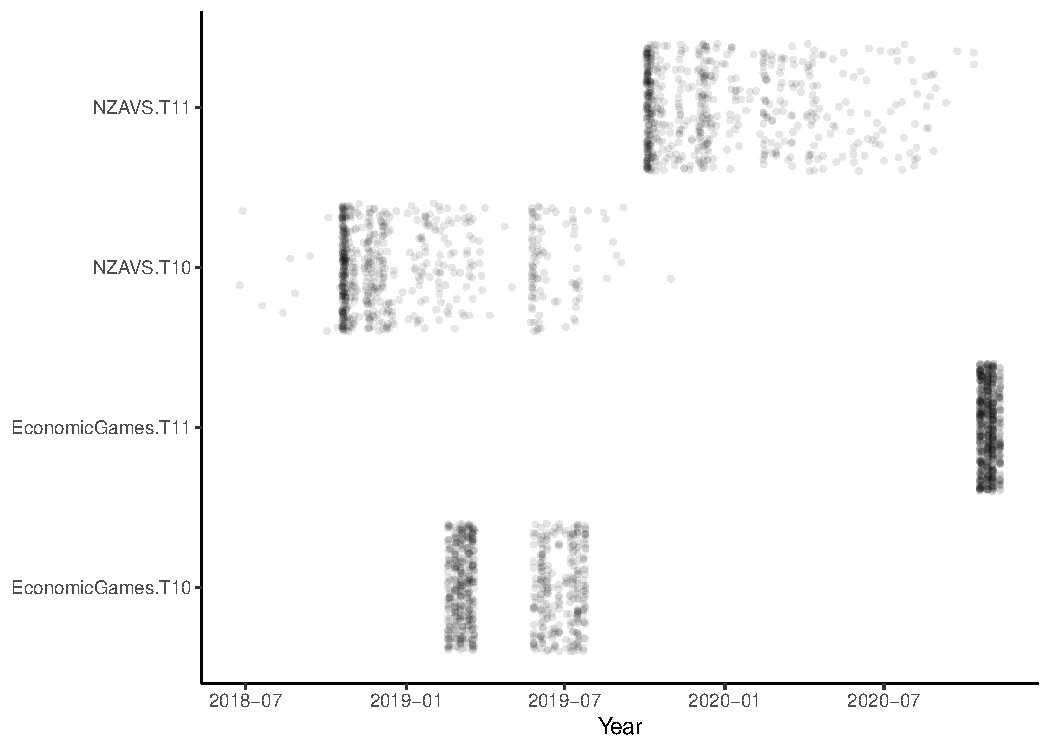
\includegraphics{manuscript_files/figure-latex/timelinePlot-1.pdf}
\caption{(\#fig:timelinePlot)(ref:timelinePlotCaption)}
\end{figure}

\newpage

(ref:impPlotCaption) \emph{Density plots showing imputed values from 20
multiply imputed datasets (pink) against observed values (blue).} Data
were imputed using predictive mean matching.

\begin{figure}
\centering
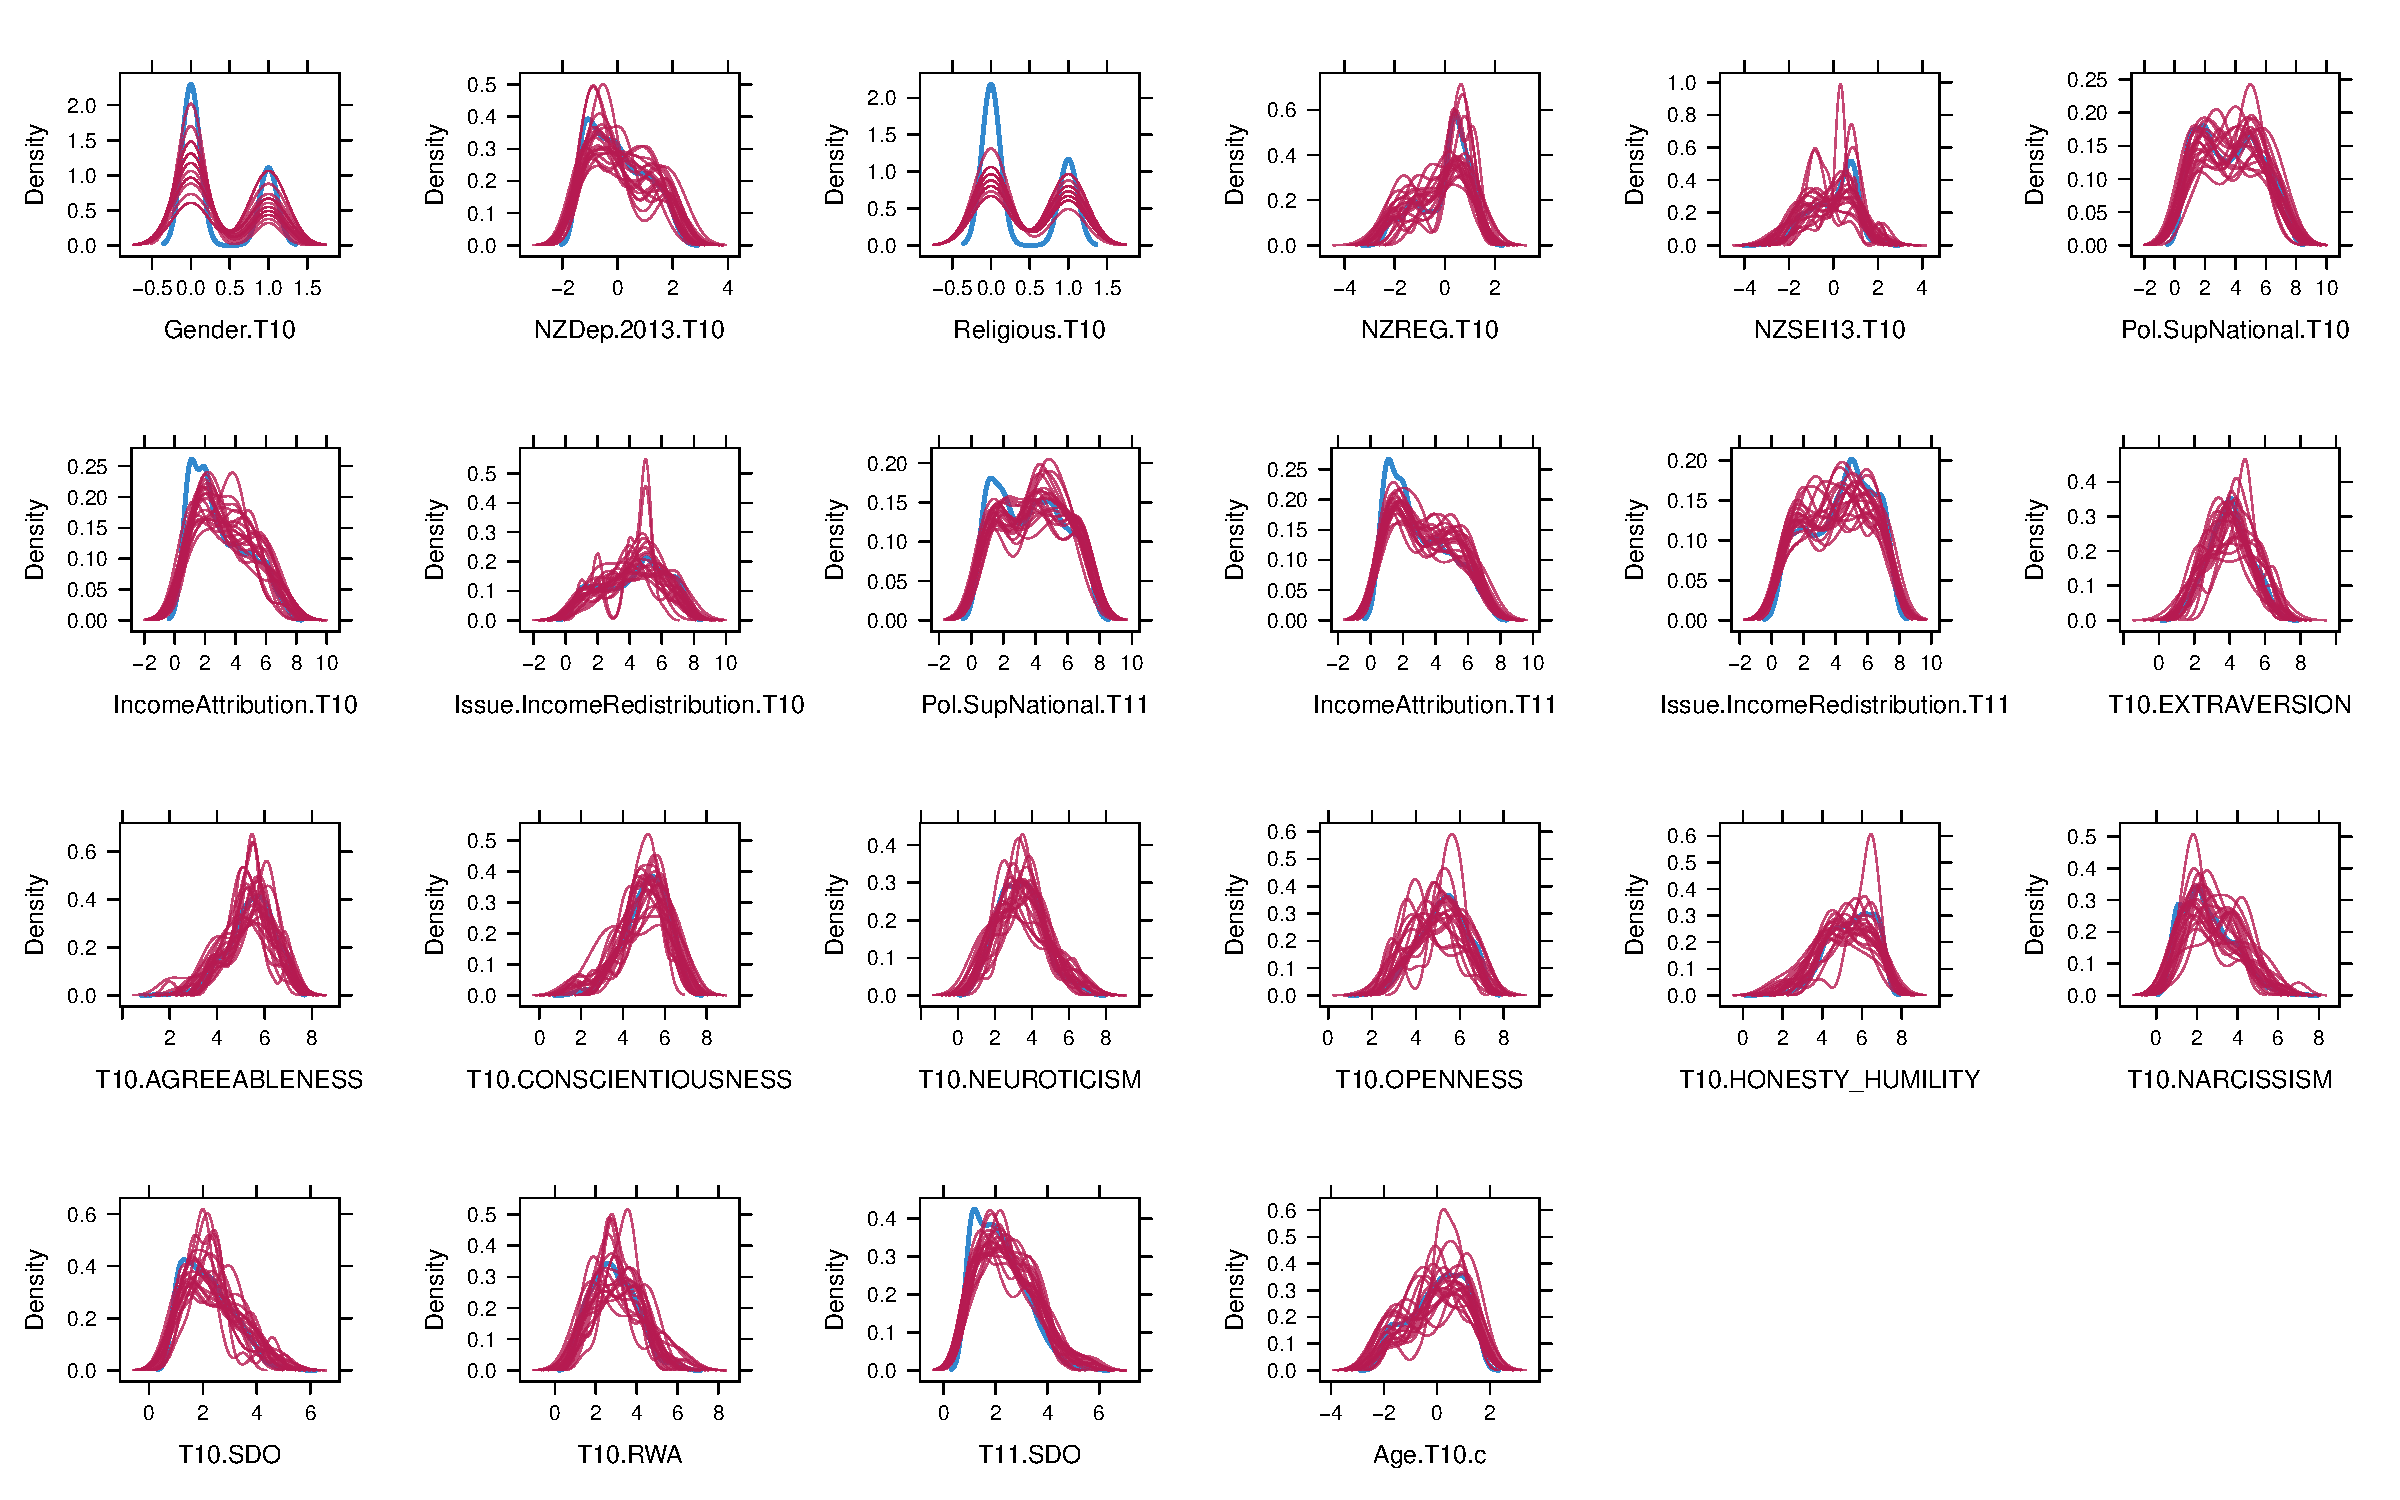
\includegraphics{manuscript_files/figure-latex/impPlot-1.pdf}
\caption{(\#fig:impPlot)(ref:impPlotCaption)}
\end{figure}

\newpage

(ref:cfa1PlotCaption) \emph{Confirmatory factor model for the
cooperative phenotype in Wave 2.} TG1 is treated as a binary endogenous
variable, and the path for TG1 is constrained to 1. Numbers are
unstandardised coefficients. *\emph{p} \textless{} 0.05. TG1 = Trust
Game (Give), TG2 = Trust Game (Return), PGG = Public Goods Game, DG =
Dictator Game.

\begin{figure}
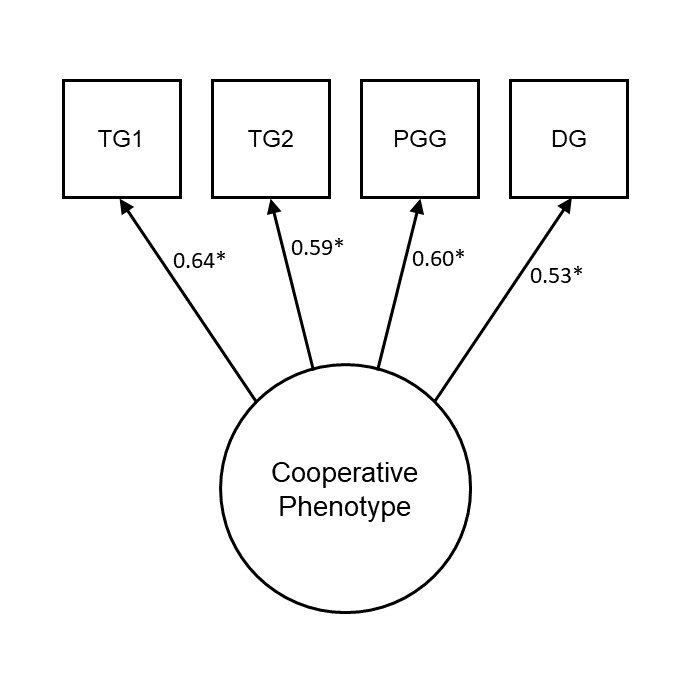
\includegraphics[width=0.8\linewidth]{modelDrawing/cfa1} \caption{(ref:cfa1PlotCaption)}(\#fig:cfa1Plot)
\end{figure}

\newpage

(ref:sem1PlotCaption) \emph{Social Dominance Orientation (mean score) is
negatively related to model-predicted cooperation latent variable
scores.}

\begin{figure}
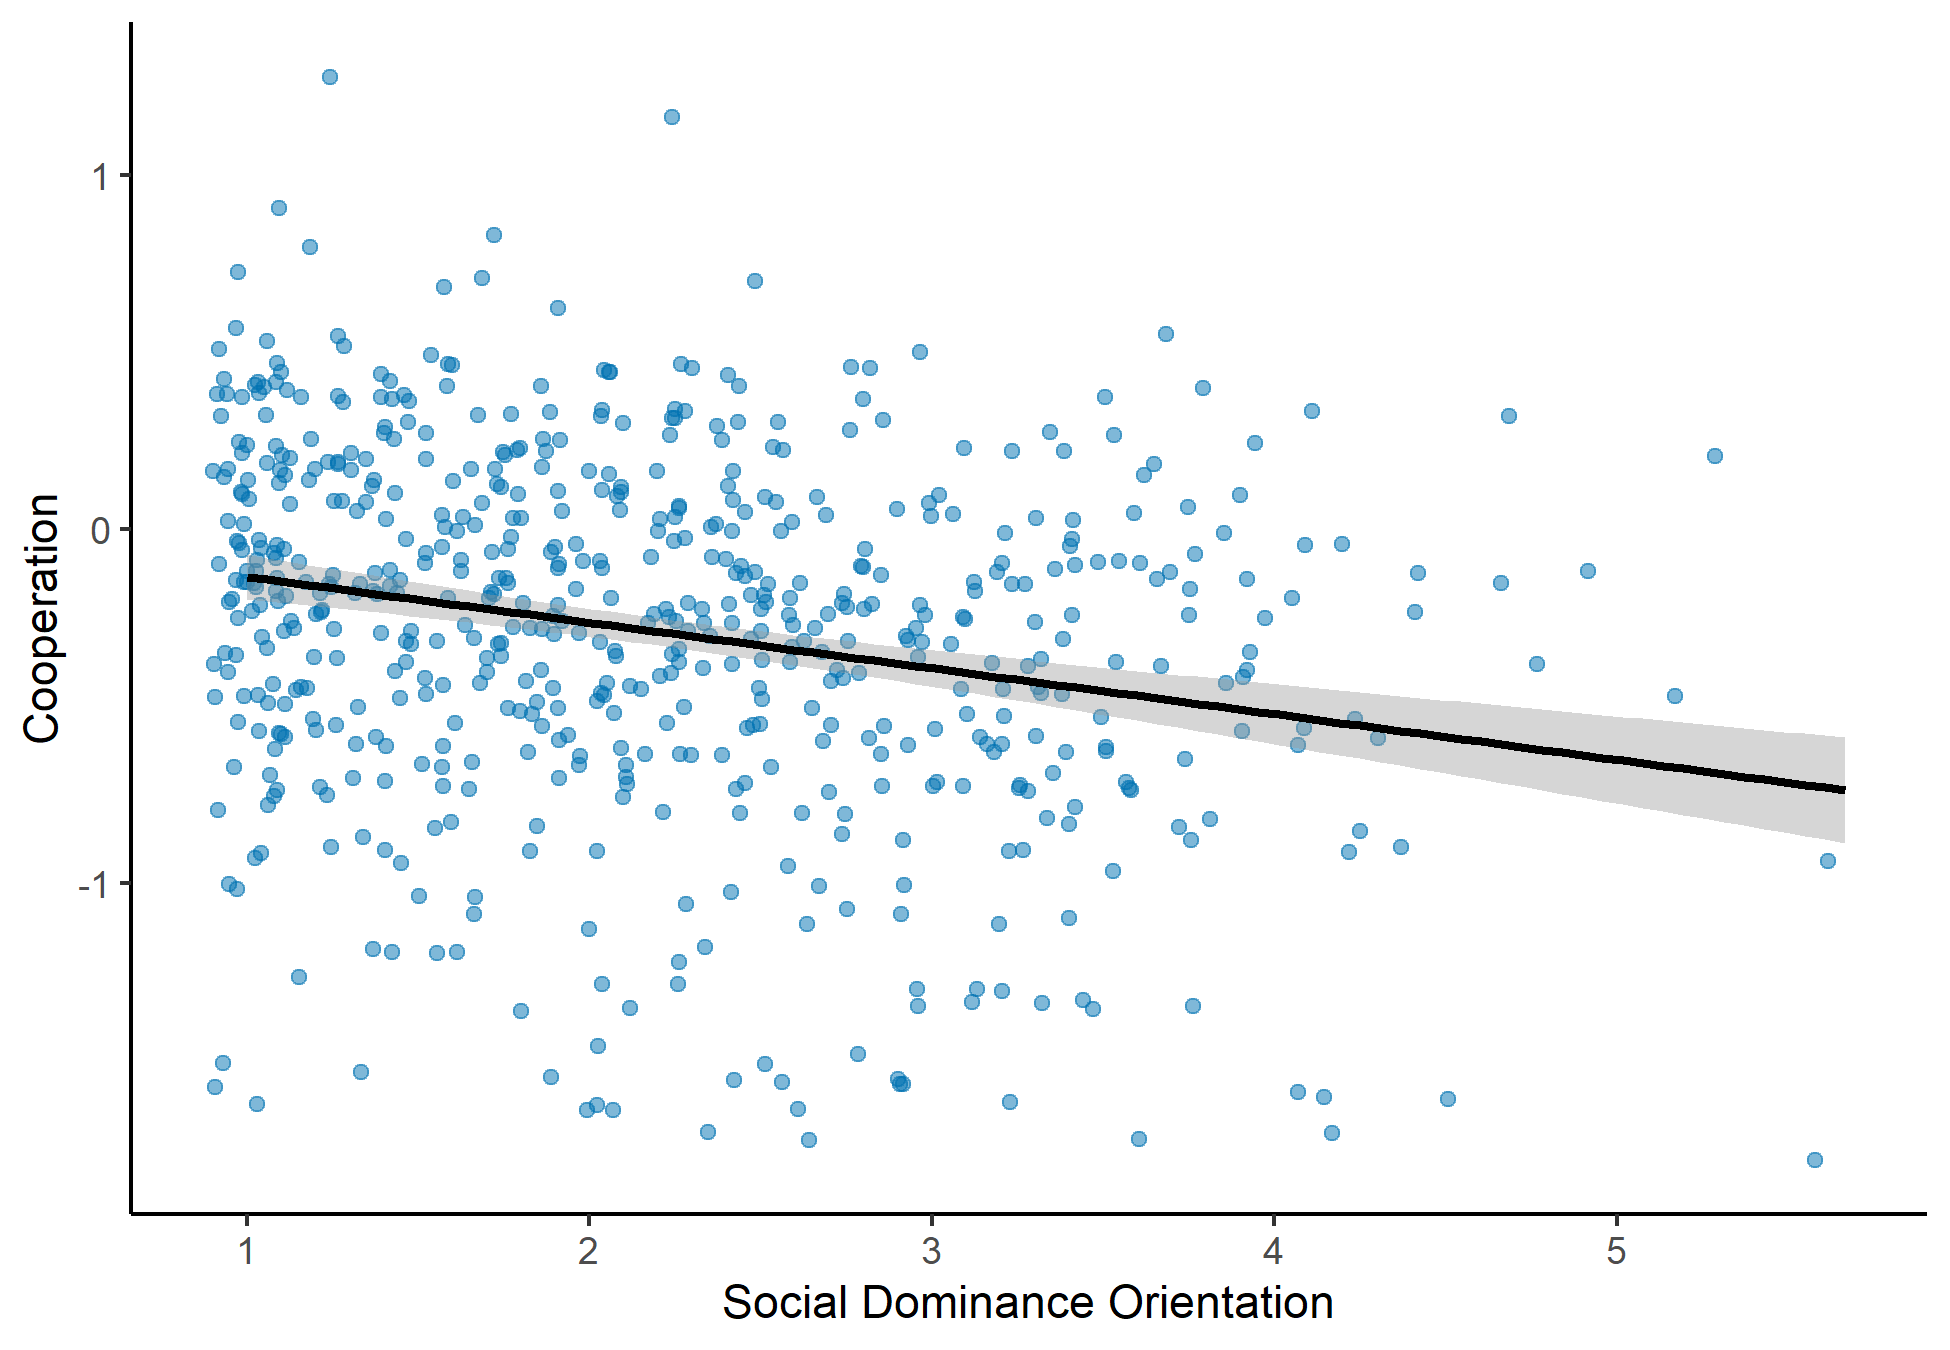
\includegraphics[width=0.8\linewidth]{manuscript_files/figure-latex/sem1Plot-1} \caption{(ref:sem1PlotCaption)}(\#fig:sem1Plot)
\end{figure}

\newpage

(ref:clpmPlotIncRedCaption) \emph{The cooperative phenotype predicts
later support for income redistribution.} (a) Cross-lagged panel model
with the cooperative phenotype and support for income redistribution.
Support for income redistribution is treated as ordinal. Note that
measurement models for the cooperative phenotype latent variables are
omitted from this figure. Numbers are standardised coefficients,
*\emph{p} \textless{} 0.05. (b, c) Forest plots visualising the change
in cross-lagged paths when controlling for time-invariant covariates,
individually and in a full model. Points are unstandardised estimates,
lines are 95\% confidence intervals.

\begin{figure}
\centering
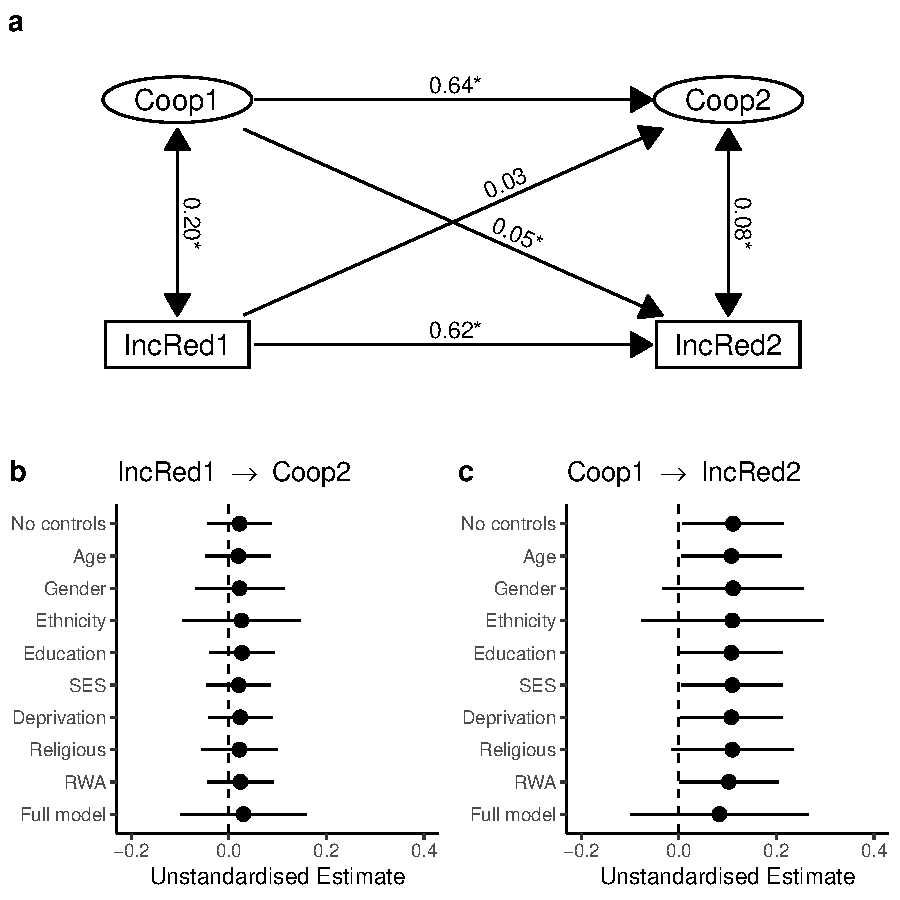
\includegraphics{manuscript_files/figure-latex/clpmPlotIncRed-1.pdf}
\caption{(\#fig:clpmPlotIncRed)(ref:clpmPlotIncRedCaption)}
\end{figure}

\newpage

(ref:clpmPlotIncAttCaption) \emph{The cooperative phenotype and income
attribution beliefs do not predict one another over time.} (a)
Cross-lagged panel model with the cooperative phenotype and income
attribution beliefs. Income attribution beliefs are treated as ordinal.
Note that measurement models for the cooperative phenotype latent
variables are omitted from this figure. Numbers are standardised
coefficients, *\emph{p} \textless{} 0.05. (b, c) Forest plots
visualising the change in cross-lagged paths when controlling for
time-invariant covariates, individually and in a full model. Points are
unstandardised estimates, lines are 95\% confidence intervals.

\begin{figure}
\centering
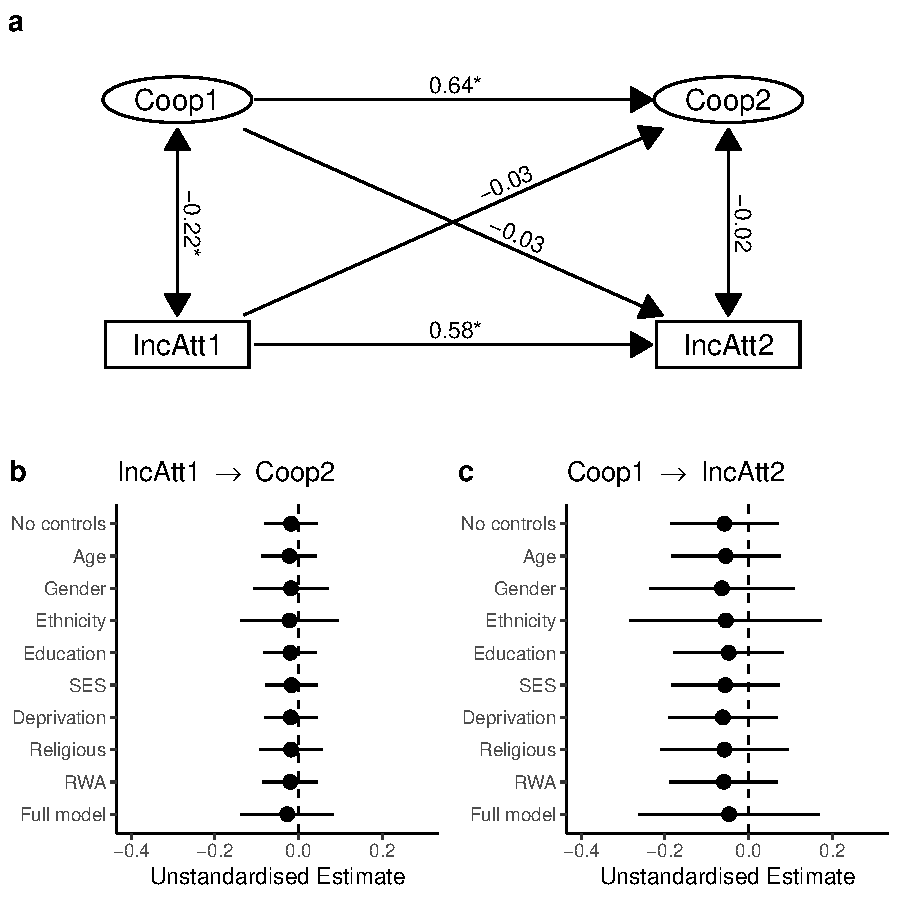
\includegraphics{manuscript_files/figure-latex/clpmPlotIncAtt-1.pdf}
\caption{(\#fig:clpmPlotIncAtt)(ref:clpmPlotIncAttCaption)}
\end{figure}

\newpage

(ref:clpmPlotPolNatCaption) \emph{The cooperative phenotype and support
for the National Party do not predict one another over time.} (a)
Cross-lagged panel model with the cooperative phenotype and support for
the National Party. Support for the National Party is treated as
ordinal. Note that measurement models for the cooperative phenotype
latent variables are omitted from this figure. Numbers are standardised
coefficients, *\emph{p} \textless{} 0.05. (b, c) Forest plots
visualising the change in cross-lagged paths when controlling for
time-invariant covariates, individually and in a full model. Points are
unstandardised estimates, lines are 95\% confidence intervals.

\begin{figure}
\centering
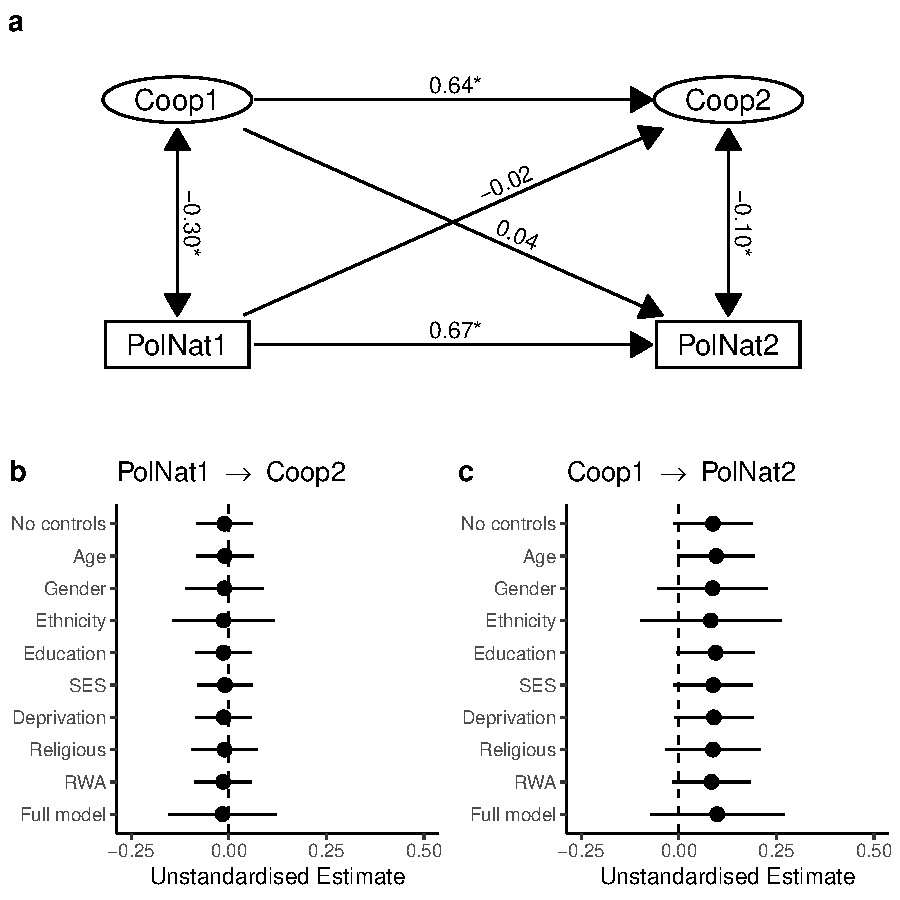
\includegraphics{manuscript_files/figure-latex/clpmPlotPolNat-1.pdf}
\caption{(\#fig:clpmPlotPolNat)(ref:clpmPlotPolNatCaption)}
\end{figure}

\newpage

\hypertarget{supplementary-tables}{%
\subsection{Supplementary Tables}\label{supplementary-tables}}

(ref:itemTableCaption) Self-report items from the New Zealand Attitudes
and Values Study.

\begin{longtable}[t]{>{\raggedright\arraybackslash}p{8em}>{\raggedright\arraybackslash}p{26em}>{\raggedright\arraybackslash}p{6em}}
\caption{(\#tab:itemTable)(ref:itemTableCaption)}\\
\toprule
Item & Description / Text & Wave\\
\midrule
SDO1 & It is OK if some groups have more of a chance in life than others & 10 - 11\\
SDO2 & Inferior groups should stay in their place & 10 - 11\\
SDO3 & To get ahead in life, it is sometimes okay to step on other groups & 10 - 11\\
SDO4 (reversed) & We should have increased social equality & 10 - 11\\
SDO5 (reversed) & It would be good if groups could be equal & 10 - 11\\
\addlinespace
SDO6 (reversed) & We should do what we can to equalise conditions for different groups & 10 - 11\\
RWA1 & It is always better to trust the judgment of the proper authorities in government and religion than to listen to the noisy rabble-rousers in our society who are trying to create doubt in people's minds & 10\\
RWA2 & It would be best for everyone if the proper authorities censored magazines so that people could not get their hands on trashy and disgusting material & 10\\
RWA3 & Our country will be destroyed some day if we do not smash the perversions eating away at our moral fibre and traditional beliefs & 10\\
RWA4 (reversed) & People should pay less attention to The Bible and other old traditional forms of religious guidance, and instead develop their own personal standards of what is moral and immoral & 10\\
\addlinespace
RWA5 (reversed) & Atheists and others who have rebelled against established religions are no doubt every bit as good and virtuous as those who attend church regularly & 10\\
RWA6 (reversed) & Some of the best people in our country are those who are challenging our government, criticizing religion, and ignoring the 'normal way' things are supposed to be done & 10\\
Income redistribution & Redistributing money and wealth more evenly among a larger percentage of the people in New Zealand through heavy taxes on the rich & 10 - 11\\
Income attribution & If incomes were more equal, people would be less motivated to work hard & 10 - 11\\
Support for National Party & Level of support for The National Party & 10 - 11\\
\addlinespace
Age & What is your date of birth? & 10\\
Gender & What is your gender? (open-ended) & 10\\
Ethnicity & Which ethnic group do you belong to? (NZ census question) & 10\\
Education level & NZ Reg (0-10 education ordinal rank) & 10\\
Socio-economic status & NZSEI13 (NZ Socio-economic index) & 10\\
\addlinespace
Local deprivation & Deprivation score 2013 (for Meshblock) & 10\\
Religiosity & Do you identify with a religion and/or spiritual group? & 10\\
\bottomrule
\end{longtable}
\end{appendix}
